\documentclass[11pt,onecolumn]{IEEEtran}
\usepackage{diagbox}
\usepackage{graphicx}
\usepackage{amsmath}
\usepackage{amsfonts}
\usepackage{algpseudocode}
% \usepackage{algorithm}
\usepackage{subfigure}
\usepackage{tikz}
\usepackage{epsfig}
\usepackage{cite}
\usepackage[linesnumbered,ruled]{algorithm2e}

\newtheorem{theorem}{Theorem}
\newtheorem{proposition}{Proposition}
\newtheorem{definition}{Definition}
\newtheorem{lemma}{Lemma}
\newtheorem{corollary}{Corollary}
\newtheorem{example}{Example}


\renewcommand{\ae}[1]{{\color{red}{#1}}}
\newcommand{\my}[1]{{\color{blue}{#1}}}
\newcommand{\old}[1]{{\color{green}{#1}}}
\newcommand{\pur}[1]{{\color{purple}{#1}}}





\begin{document}     
\title{Prediction Uncertainty Based On Classification Agianst Unmodelled Input Space}
\author{Xiaozhe Gu\\Energy Research Institute (ERI@N), Singapore }

\maketitle

\section{Basic Decision Tree}
\begin{itemize}
  \item Criterion: Gini Index
\begin{align*}
I_G(p)=\sum_{i=1}^np_i(1-p_i)=1-\sum_{i=1}^n p_i^2
\end{align*}
\item Split Value for feature j: $\mathbf X_j\in  \{\mathbf X_{1,j},\mathbf X_{2,j},\ldots,\mathbf X_{n,j}\}$. We do not need to consider the value in empty space.
\item Gini Index After Split by feature i and value s $R_1(x_i,s)=\{x|x_i\leq s\}$, and $R_1(x_i,s)=\{x|x_i>s\}$,$s \in \mathbf X_j$:
\begin{align*}
IG_L(x_i,s)=1-\left(\frac{R_1(x_i,s)}{R_1(x_i,s)+E_1}\right)^2-\left(\frac{E_1}{R_1(x_i,s)+E_1}\right)^2\\
E_1=E\times \left(\frac{s-x_i^{\mbox{min}}}{x_i^{\mbox{max}}-x_i^{\mbox{min}}}\right)\\
IG_R(x_i,s)=1-\left(\frac{R_2(x_i,s)}{R_2(x_i,s)+E_2}\right)^2-\left(\frac{E_2}{R_1(x_i,s)+E_2}\right)^2\\
E_2=E\times \left(\frac{x_i^{\mbox{max}}-s}{x_i^{\mbox{max}}-x_i^{\mbox{min}}}\right)\\
E=R\times c,\mbox{ where c is a hyper paramter}\\ 
IG_{\mbox{gain}}(x_i,s)=\frac{R_1+E_1}{R+E}IG_L+\frac{R_2+E_2}{E+R}IG_R\\
x_i,s=\arg \min_{x_i,s} IG_{\mbox{gain}}(x_i,s)
\end{align*}
\item Node Representation after spilt: the limit of each feature in the split data:  $[x_i^{\mbox{min}},x_i^{\mbox{max}}]$ for each i.  Any x that not include in these rules are consider empty. 
  \begin{figure}[h]
    \centering
    \caption{Tree Representation}
    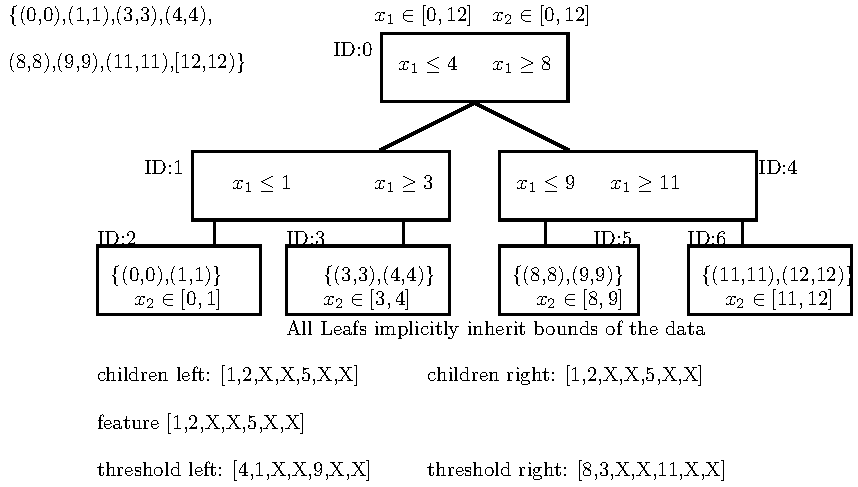
\includegraphics[scale=1]{image/tree.pdf} 
    \end{figure}
\begin{itemize}
    \item why still use tree not rules directly? The features are used  find the decision path for predicting faster. Suppose $x=(0.5,0.5)$, the decision procedure is that : node 0, feature[0],threshold left[0],children left[0]=1, node 1, feature[1],threshold left[1],children left[1]=2, node=2,feature[2]=X, node 2=Leaf. 
    \item  Furture work:  But $x_i^{\mbox{min}},x_i^{\mbox{max}}$ can be manually set to avoid the case that $X_i$ is amostly uniformaly distributed. Thus $\mu(x_{i,k+1}-x_{i,k}))$ is a useful information to determine the node limitations. For now, just let bagging solve these problems.
\end{itemize}
 

\item For category feature, for example, $X_i\in\{1,2,3,4,5\}$, we do not need to consider these features.


\end{itemize}



\subsection{Issues}
\begin{itemize}
	\item Suppose for node 0, the split feature index is i, with data $\{1,2,4,7,10\}$ and s=4, then the left is $x_i\leq 4$ and the right is $x_i>4\Rightarrow x_i\geq 7$. Thus, we \texttt{ node 0} should restore  \texttt{feature i, sl=4,sr=7}.
	\item The edge limit of each split is stored in the data structure, and the leafs.
    \item Stop  building when  \texttt{n\_sampling=1} , and at this time, the confident region is around the data point $x$
    \item \textbf{Problem:} how to determine the \texttt{n\_sampling}  after each split is a big question.  Suppose $x_1=2 x_2+b+\sigma^2$, then \texttt{n\_empty >>n\_sampling} 
\end{itemize}



\subsection{Ideas}:
\begin{itemize}
	\item  Also consider the feature importance. For example, feature 1 is important when $x_1\in[0,10]$, then, as we consider the split feature, this feature could has higher priority
	\item Consider the problem to classify 100 points in 10 dimension.
    \item consider the variance of data in the split?  If it has small variance, then reduce the empty samples?
\end{itemize}

% \renewcommand{\refname}{~}
% \begin{thebibliography}{1}

% \bibitem{safeml} Varshney KR, Alemzadeh H. On the safety of machine learning: Cyber-physical systems, decision sciences, and data products. Big data. 2017 Sep 1.



% \bibitem{lime} Ribeiro, Marco Tulio, Sameer Singh, and Carlos Guestrin. Why should i trust you?: Explaining the predictions of any classifier. Proceedings of the 22nd ACM SIGKDD International Conference on Knowledge Discovery and Data Mining. ACM, 2016.


% \bibitem{reject} Bartlett P L, Wegkamp M H. Classification with a reject option using a hinge loss[J]. Journal of Machine Learning Research, 2008, 9(Aug): 1823-1840.

% \bibitem{errorbound} K. R. Varshney, R. J. Prenger, T. L. Marlatt, B. Y. Chen, and W. G. Hanley, Practical ensemble classification error bounds for different operating points, IEEE Transactions on Knowledge and Data Engineering, vol. 25, no. 11, pp. 2590-2601, Nov. 2013.
% \bibitem{nntogp} Gal Y, Ghahramani Z. Dropout as a Bayesian approximation: Representing model uncertainty in deep learning[C]//international conference on machine learning. 2016: 1050-1059.

% \bibitem{abstract} Tommaso Dreossi, Alexandre Donze,  Sanjit A. Seshia, Compositional Falsification of Cyber-Physical Systems with Machine Learning Components, Preprint

% \bibitem{bnn12} Neal, R. M. (2012). Bayesian learning for neural networks (Vol. 118). Springer Science \& Business Media.
%

% \bibitem{Amodei} Amodei, Dario, Chris Olah, Jacob Steinhardt, Paul Christiano, John Schulman, and Dan Mane. 2016. Concrete Problems in AI Safety.

% \bibitem{Bostrom} Bostrom, N., Dafoe, A., and Flynn, C. 2016. Policy Desiderata in the Development of Machine Superintelligence


% \bibitem{conform} Vovk V, Gammerman A, Shafer G. Conformal prediction[M]. Springer US, 2005

% \bibitem{towardverify}  S. A. Seshia, D. Sadigh, and S. S. Sastry. Towards verified artificial intelligence. CoRR, abs/1606.08514, 2016.
 


% \bibitem{reduce} Weiming Xiang and Taylor T. Johnson, Reachability Analysis and Safety Verification for Neural  Network Control Systems,Preprint.


 



% \end{thebibliography}


\end{document}
